\title{Projeto Biblioteca Espectral de Solos do Brasil - BESB}
\author{por José Alexandre M. Demattê e Marilusa P. C. Lacerda}
\maketitle

A população mundial compreende, atualmente, cerca de 7.207.456 bilhões de pessoas e é esperado um valor de 8.612.262 até 2050, segundo dados da \citet{FAO:2013}. Como alimentar essa população? Em 2006, na Conferência Mundial em Infra-estrutura Geospacial e banco de dados, ocorrida no Chile, com 63 países participantes, concluiu-se que para atender as necessidades da população mundial crescente nesta proporção, será necessária a elaboração de mapas temáticos dos recursos naturais em escalas detalhadas (entre eles solos), bem como a organização dos dados relacionados em bancos de dados digitais, como forma de subsidiar o planejamento das atividades agrícolas e produção de alimentos. Afora o lado da necessidade humana, destaca-se a importância do agronegócio no Brasil. Do valor bruto da produção do agronegócio brasileiro, que chegou a R\$470 bilhões em 2013, 66\% refere-se à agricultura. Somente a China, em 2013, comprou do Brasil US\$23 bilhões só em alimentos, e das exportações totais de soja nos próximos 10 anos, 71,3\% devem ser dirigidas para a China \citep{Brasil:2013}. Estes dados mostram a força do Brasil na agricultura e na economia mundial.\\
\\
\begin{figure}[htbp]
   \centering
   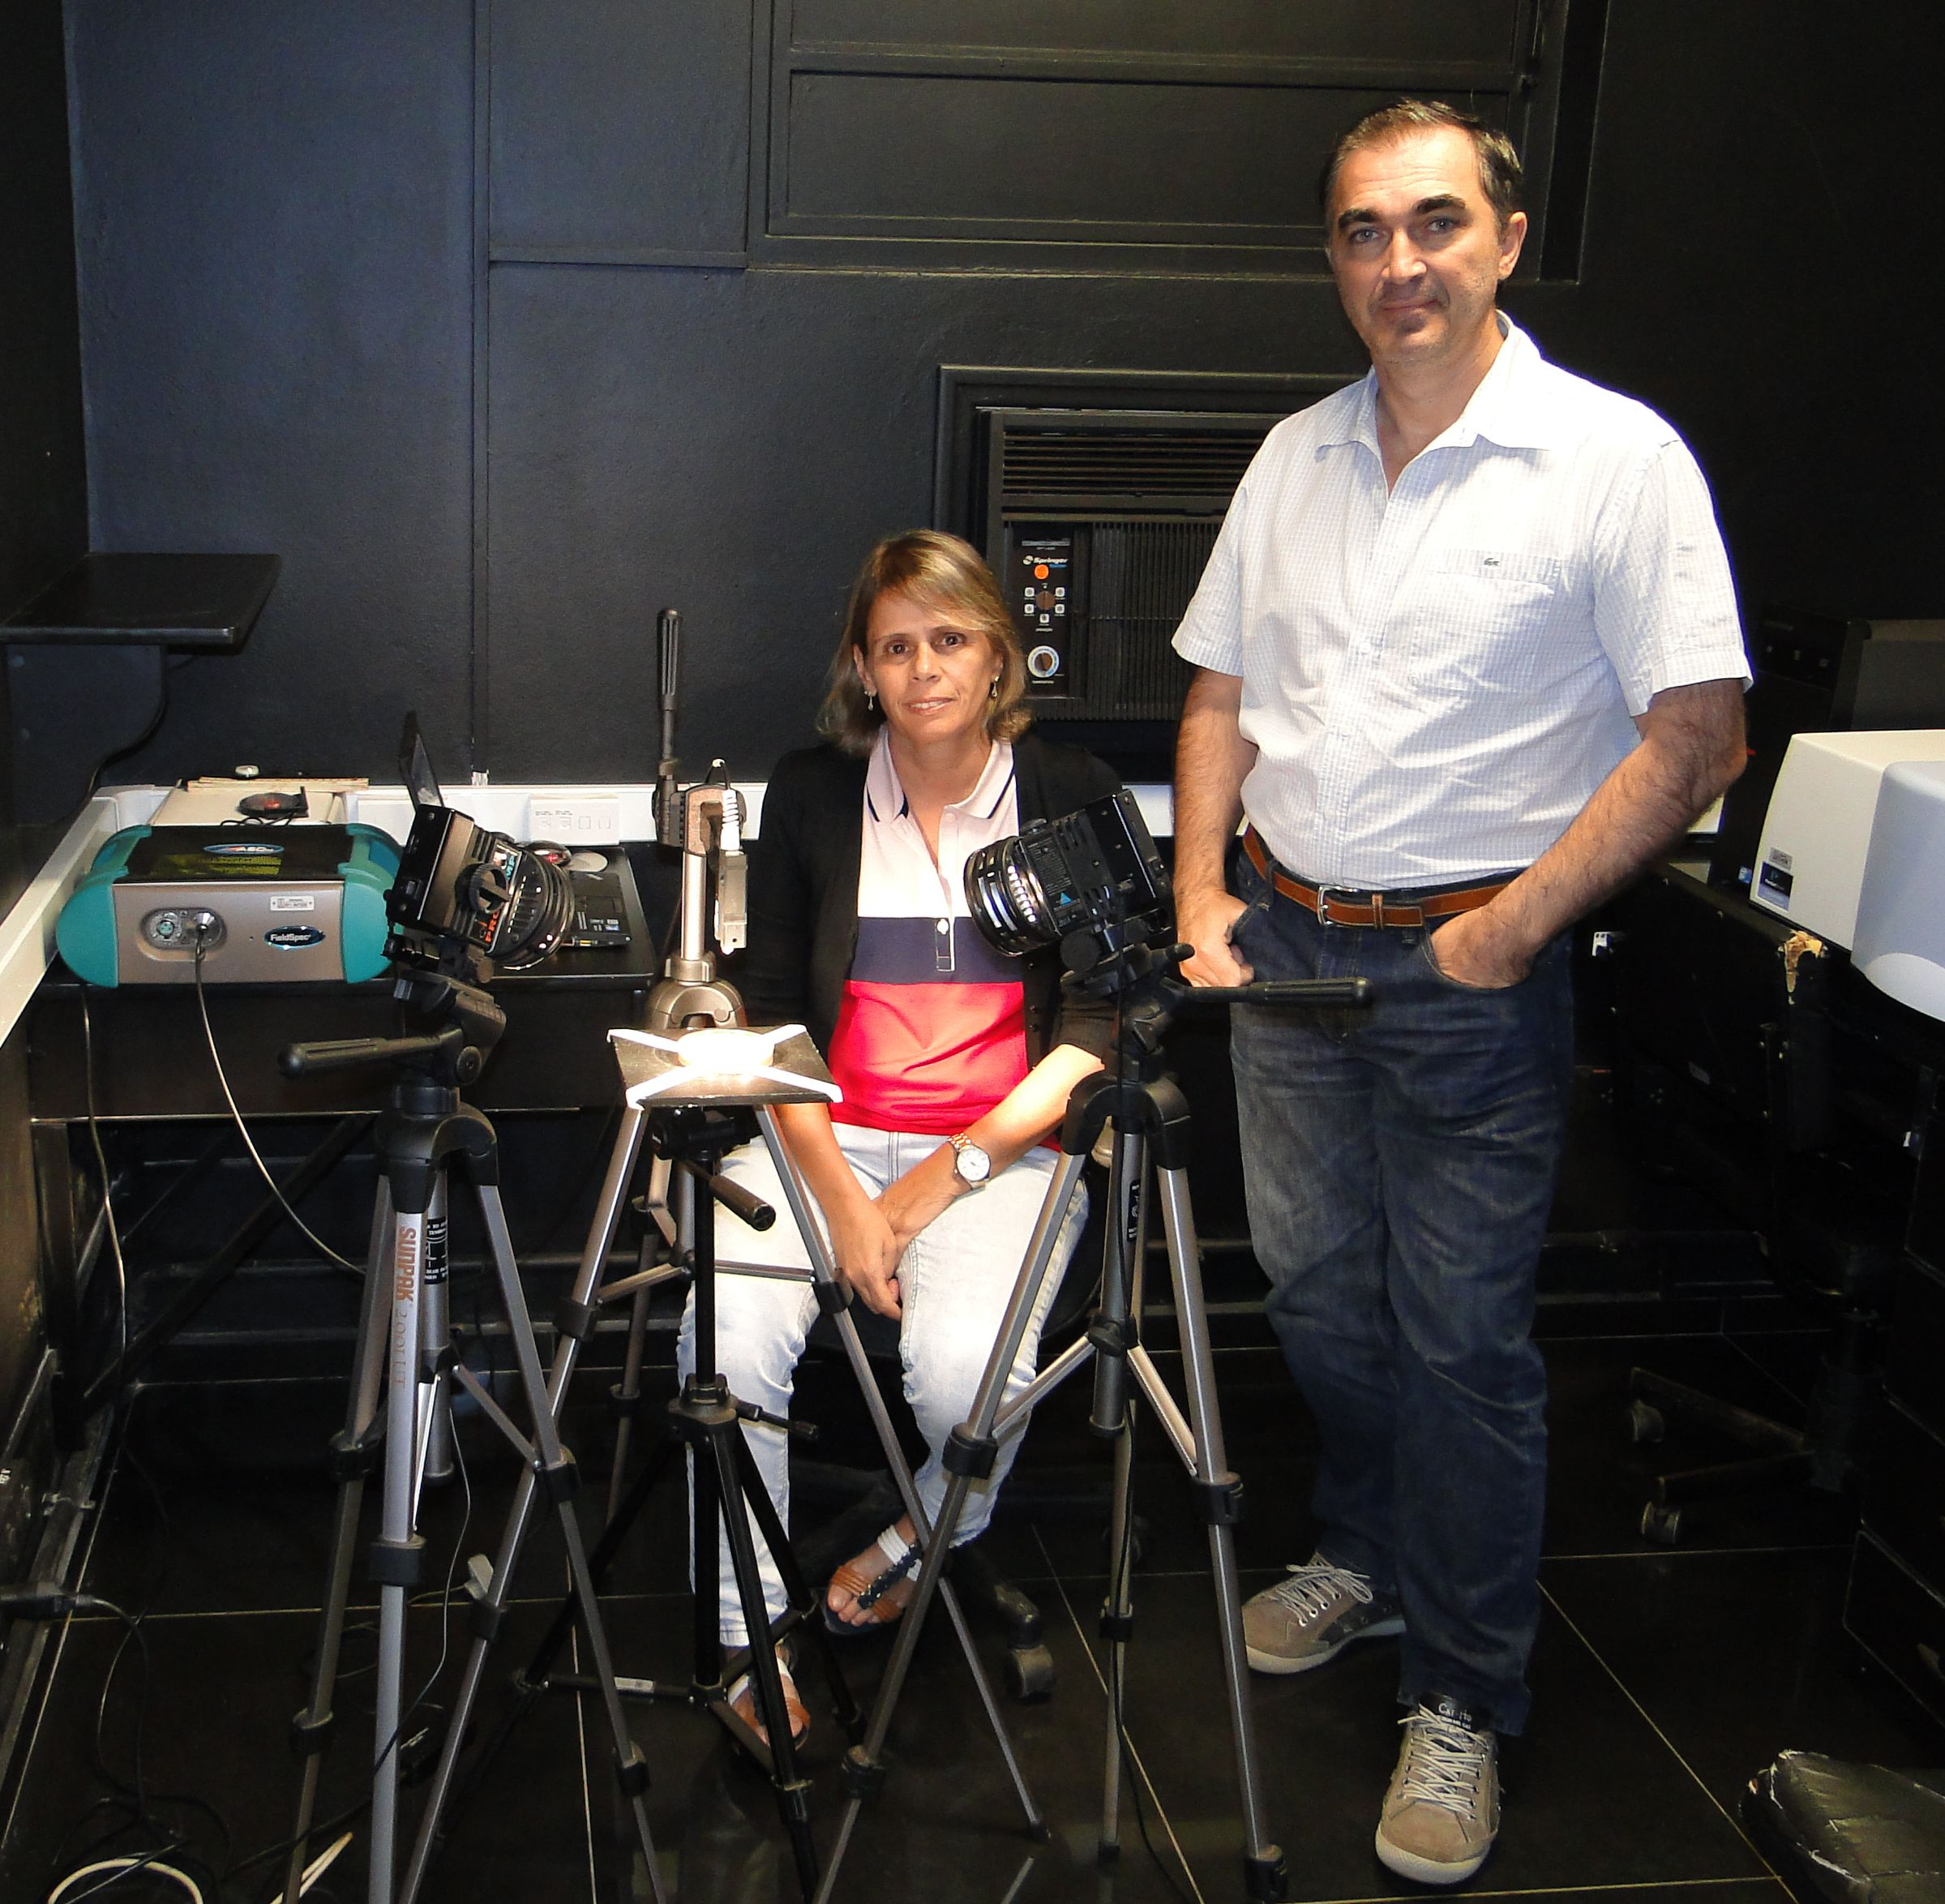
\includegraphics[width=0.8\textwidth]{figuras/dematte-marilusa.jpg}
   \caption{Os autores no Laboratório de Sensoriamento Remoto e Geoprocessamento Aplicado a Solos e Uso da Terra do Departamento de Ciência do Solo da Escola Superior de Agricultura Luiz de Queiroz.}
   \label{fig:autores}
\end{figure}

Por outro lado, apesar de precisarmos do solo, não o tratamos adequadamente. \citet{Mahmood:1987} já destacava a grande perda de solos pelas atividades antrópicas sem planejamento adequado, por intermédio do elevado acúmulo de sedimentos nos reservatórios de água do mundo. A maioria da literatura disponível mostra que o transporte anual de sedimentos, incluindo solos erodidos, para os oceanos pelos rios do mundo, é de 15-20 bilhões de Mg de acordo com \citet{Lal:2003}. O uso de herbicidas no solo varia de g a kg nos Estados Unidos e vários outros países desenvolvidos, causando sérios problemas aos solos e lençóis freáticos \citep{SinghEtAl:2010}. A ocorrência de CO$_2$ na atmosfera aumentou em 36\% entre 1750 e 2006 \citep{CoelhoEtAl:2013}, causado pelo uso inadequado dos solos. Os solos tem importância nos teores de carbono orgânico e inorgânico, que por sua vez tem relação com as questões atmosféricas e climáticas \citep{Lal:1999}.

\subsection*{Como evitar e solucionar estes problemas?}

Conhecer os solos, seus atributos e sua espacialidade estão intimamente relacionados ao apoio na resolução de vários dos problemas apontados. O conhecimento espacializado dos solos podem auxiliar em: conservação do solo, planejamento do uso da terra, alocação varietal, planejamento experimental, planejamento em manejo de solo (aração, gradagem, descompactação, entre outros), manejo dos ambientes (épocas de plantio, colheita), planejamento paisagístico, urbanos, na área de engenharia, entre inúmeras outras funções. Basta saber usar.

O Brasil teve grandes avanços em mapeamentos pedológicos realizados nas décadas de 70 e 80, mas a escala de pouco detalhamento utilizada permitiu somente avaliações estratégicas e não são adequados para o nível agrícola atual. Por outro lado, para a real importância destes mapas para a expansão da agricultura em grandes proporções são necessários mapas de solos em níveis detalhados em grandes escalas (faixa de 1:20.000). Neste quesito, estamos ``a pé'' e longe da real necessidade do país. Na realidade, o Brasil possui, no máximo, 0,25\% do seu território com mapas pedológicos detalhados ou semi-detalhados \citep{Mendonca-SantosEtAl:2007}.

\subsection*{O uso de Sensoriamento Remoto no mapeamento de solos em escalas detalhadas no Brasil}

Diante da grande extensão territorial do Brasil, falta de pessoal especializado e financiamentos de grande amplitude, somente com a agregação das geotecnologias aos métodos clássicos de levantamento e mapeamento de solos será possível atingir nosso intento. Dentre estas geotecnologias, ressalta-se o sensoriamento remoto (SR), definido basicamente como ``a aquisição de dados de um objeto sem haver contato direto com o mesmo''. Esse dado pode ser em diversos níveis de aquisição desde laboratorial, campo, aéreo e orbital. 

Para que tal tecnologia se desenvolva, é extremamente importante que entre na grade de ensino, em especial, na área de agronomia, as técnicas (dentro das quais entra o SR e o mapeamento digital) de mapeamento de solos e a sua aplicação no processo agrícola. O mapeamento é o resultado do estudo nas mais diversas áreas da ciência do solo, sendo a base no processo de planejamento agrícola. Logo, não há como fugir a inserção do aparato tecnológico na área de ensino, sob pena de perda do interesse dos alunos. Por outro lado, a base fundamental (Pedologia, gênese, trabalhos de campo) deve continuar a ser dada em consonância ao avanço tecnológico. 

A espectroscopia, metodologia associada ao SR, é uma ferramenta poderosa para a detecção e análise de alvos, baseada na interação da radiação eletromagnética (REM) com a matéria. A REM em comprimentos de onda diferentes transporta quantidades de energia diversificadas e proporcionam interações variadas entre as moléculas e os átomos que podem interagir com os fótons (ondas eletromagnéticas), absorvendo, transmitindo ou refletindo energia. A energia refletida pode ser medida por um equipamento específico, o espectrorradiômetro, definindo a espectroscopia de emissão, com medições da radiância ou reflectância da REM. O resultado é a obtenção de assinaturas ou curvas espectrais específicas de cada material analisado em vários intervalos de comprimento de onda do espectro eletromagnético, desde o Visível (400-750~nm), Infravermelho Próximo e Médio (750-2.500~nm) (Figura \ref{fig:curvas}), podendo atingir o Infravermelho Médio (2500-25000~nm). Basicamente, tal tecnologia pode e deve ser associada a metodologias matemáticas, estatísticas e geoestatísticas para atingir melhores resultados em pedotransferências. A espectroscopia se destaca por ser um procedimento rápido, não destrutivo, de menor custo e que, praticamente não proporciona impactos ambientais, quando comparado às metodologias tradicionais. Basicamente os dados espectroscópicos adquiridos têm duas funções: a) quantificar atributos de solos, tais como teores de argila, areia, Fe$_2$O$_3$, carbono orgânico, valores de Ki, CTC, entre outros \citep{Soriano-DislaEtAl:2014}; e b) a assinatura espectral de amostras dos horizontes de um perfil pedológico permite inferir a provável classe deste solo \citep{VasquesEtAl:2014}. Uma das grandes vantagens do método é que de uma única leitura e em um mesmo aparelho, pode-se diagnosticar inúmeras informações sobre o solo, como seus atributos e o padrão da curva espectral terá correlação com a provável classe de solo. Além disso, os dados espectroscópicos adquiridos em laboratório têm outros itens de importância tais como: base para o entendimento dos padrões espectrais obtidos no campo; base para a compreensão dos dados alcançados por sensores instalados em aviões e satélites; base para a compreensão dos recentes avanços de sensores hiperespectrais; meio de comunicação entre a comunidade científica (pois o espectro é igual para todos), entre outras.

\begin{figure*}[tb!]
\begin{minipage}[t]{1\linewidth}
   \centering
   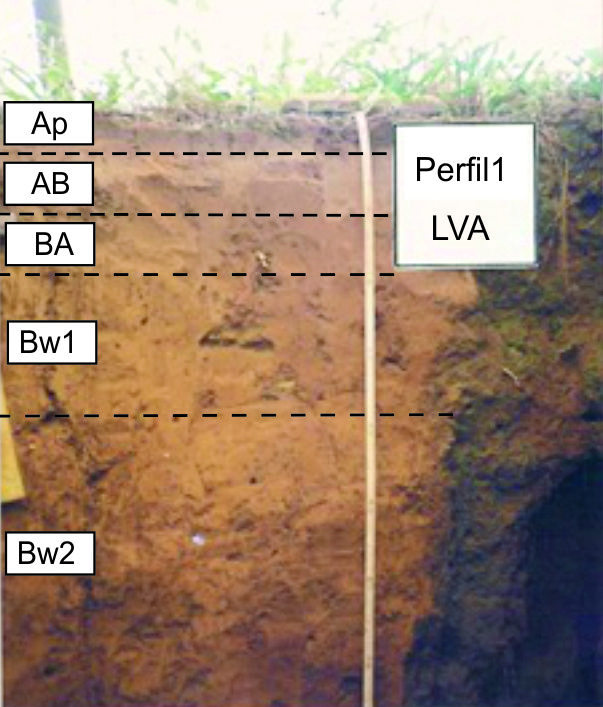
\includegraphics[width=0.49\textwidth]{figuras/lva.jpg}
   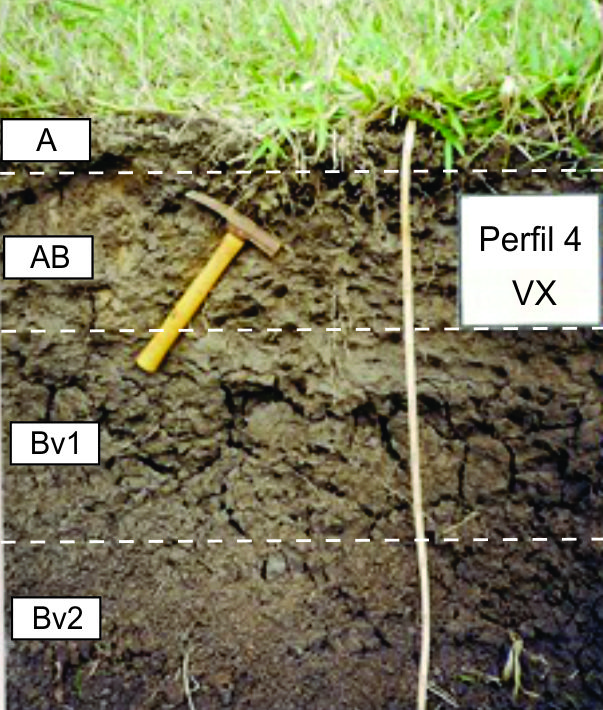
\includegraphics[width=0.49\textwidth]{figuras/vertissolo.jpg}
   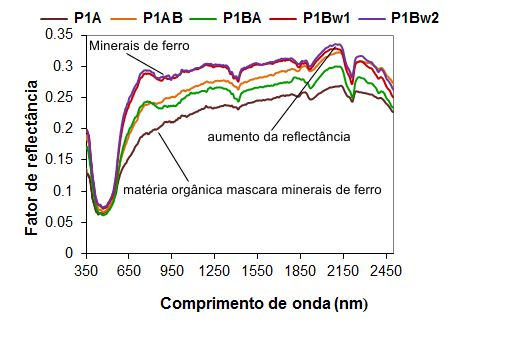
\includegraphics[width=0.49\textwidth, trim=0.5cm 0cm 1.5cm 0cm, clip]{figuras/curvas-lva.jpg}
   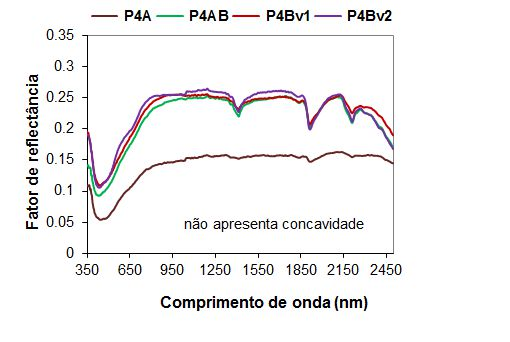
\includegraphics[width=0.49\textwidth, trim=0.5cm 0cm 1.5cm 0cm, clip]{figuras/curvas-vertissolo.jpg}
   \caption{Relações entre classes de solos e suas curvas espectrais. Solo 1 -- Latossolo Vermelho-Amarelo e curvas espectrais dos horizontes Ap, AB, BA, Bw1, Bw2. Solo 2 -- Vertissolo Háplico e curvas espectrais dos horizontes A, E, Bv1 e Bv2.}
   \label{fig:curvas}
\end{minipage}
\end{figure*}

\subsection*{Biblioteca Espectral de Solos do Brasil - BESB}

Um dos pilares para o sucesso de futuros mapeamentos de solos no Brasil é a montagem de bancos de dados de espectros de solos, aqui denominada Biblioteca Espectral de Solos do Brasil (BESB). Tal projeto trata da aquisição e armazenamento de padrões de curvas espectrais adquiridas de amostras de solos de várias regiões do Brasil. Tem por objetivos: (a) ter num único local, armazenadas informações relevantes de solos para estudos futuros; (b) realizar publicações iniciais demonstrando a utilidade desta poderosa ferramenta utilizando simultaneamente os dados de todo o Brasil; (c) estabelecer e consolidar uma comunidade que comece a entender e utilizar na prática a espectroscopia de solos; (d) ser a base para a comunidade pedológica em futuras pesquisas com adoção de novas tecnologias locais e regionais; (e) ser um pilar de apoio no mapeamento de solos; (f) ser um embasamento para o entendimento de dados obtidos por sensores aéreos e orbitais no território nacional.

Várias iniciativas têm sido realizadas no mundo desde \citet{StonerEtAl:1981}, até \citet{ShepherdEtAl:2002}, e \citet{BrownEtAl:2006}. No Brasil, o trabalho pioneiro foi de \citet{EpiphanioEtAl:1992}, publicado por \citet{FormaggioEtAl:1996} para o estado de São Paulo. Posteriormente, e com o objetivo de demonstrar a aplicação em mapeamento de solos, o primeiro trabalho realizado para cinco estados nacionais foi feito por \citet{BellinasoEtAl:2010}. A aplicação da técnica de sensoriamento remoto aplicada em mapeamento de solos foi descrita pela primeira vez no Brasil em 2004 por \citet{DematteEtAl:2004}, os quais seguiram a metodologia tradicional, porém aplicando os conceitos de espectroscopia. Em adição a isso, \citet{DematteEtAl:2001} já haviam associado a metodologia tradicional com fotos aéreas e espectroscopia, atingindo 90\% de coincidência com um trabalho realizado utilizando unicamente as técnicas tradicionais de levantamento e mapeamento de solos. Isso nos leva a outras aplicações de importância relevante nas Ciências Agrícolas, Ambientais e Agricultura de Precisão \citep{ThomassonEtAl:2001, OdlareEtAl:2005}. Na Europa, um grande projeto denominado \href{http://eusoils.jrc.ec.europa.eu/projects/Lucas/}{LUCAS} (Land Use/Cover Area frame Statistical Survey) foi elaborado na forma de banco de dados em 2013 com 20.000 amostras de solos recobrindo 23 países. Porém, o foco desta biblioteca está na quantificação dos solos e não classificação. Em contrapartida, outro projeto em andamento iniciado em 2008 compreende a participação de 80 países com a criação de um grupo em espectroscopia de solos, coordenado por \href{http://groups.google.com/group/soil-spectroscopy}{Viscarra Rossel}, relacionando as amostras de solos com classes e atributos dos mesmos \citep{ViscarraRossel:2009}.

Devido a tudo isso, foi proposta a primeira Biblioteca do Brasil, BESB (\url{http://bibliotecaespectral.wix.com/esalq}), cujas pesquisas estão sendo coordenadas pelo Prof. José Alexandre M. Demattê e pelo Grupo de Pesquisas em Geotecnologia em Ciência do Solo (\href{http://esalqgeocis.wix.com/geocis}{GeoCis}) no Laboratório de Sensoriamento Remoto e Geoprocessamento Aplicado a Solos e Uso da Terra do Departamento de Ciência do Solo da Escola Superior de Agricultura Luiz de Queiroz (ESALQ-USP) (Figura \ref{fig:autores}). Este projeto está vinculado ao já criado Grupo de Pesquisa em Espectroscopia de Solos do Brasil (GESB) pelo CNPq. Tal projeto atualmente conta com a colaboração de pesquisadores de dezenas de instituições parceiras, como a Empresa Brasileira de Pesquisa Agropecuária (Embrapa), o Instituto Agronômico de Campinas e diversas Universidades Estaduais e Federais, com representantes da Rede de Mapeamento Digital de Solos do Brasil (RedeMDS).

Até o momento, a Biblioteca Espectral de Solos do Brasil já reuniu informações de dez estados, com 14.839 amostras de solos já processadas e várias outras sendo preparadas para análises. Destas, 90\% pertencem ao acervo do Departamento de Ciência do Solo, oriundas de pesquisas diversas coordenadas pelo Prof. Demattê, sendo as demais cedidas por parceiros externos.

Atualmente, a Biblioteca está sendo desenvolvida por meio de aquisição de dados analíticos de atributos químicos básicos dos Solos (principalmente, matéria orgânica e/ou carbono, P, Ca, Mg, K, Al, H, pH, V\%, m\% e CTC), análises granulométricas (teores de areia, silte e argila) e curvas espectrais obtidas na faixa de comprimento de onda de 400-2500 nm por meio do equipamento denominado ASD Fieldspec. Para algumas amostras pretende-se obter dados em 2500-25.000~nm.

\subsection*{Como colaborar e utilizar a BESB?}

Toda a comunidade da Ciência do Solo do Brasil foi convidada a colaborar por meio de envio de amostras de solos de suas regiões. Para participar basta entrar no site da BESB e ver o protocolo. Resumidamente, os interessados devem: enviar amostras de perfis completos (com a designação dos horizontes), analises mínima química e granulométrica, classificação do solo e devem informar o local de coleta, preferencialmente com latitude e longitude (caso não seja possível, com o nome do município mais próximo). Como segunda opção, pode-se enviar amostras coletadas com trado, porém que se tenha, no mínimo, as camadas 0-20 e 80-100~cm no mesmo ponto, para que permita ter a variação analítica entre camadas. Informar a provável classificação do solo e demais informações da mesma forma que nos perfis. A quantidade de terra a ser enviada é de mínimo 50~g, secas, moídas e peneiradas (2~mm). Quem não tiver o equipamento, enviar para a ESALq que faremos as leituras e devolveremos os resultados. Se a instituição cedente tiver espectroradiômetro pode enviar diretamente as curvas espectrais para a ESALq, cujos resultados serão implementados no banco de dados, dentro do servidor do Laboratório de Sensoriamento Remoto e Geoprocessamento aplicado a Solos e Uso da Terra do Departamento de Ciência do Solo da ESALq-USP. O banco de dados já conta com amostras de estados como São Paulo, Goiás, Mato Grosso do Sul, Paraná, Minas Gerais, Rio Grande do Sul, Pernambuco, Pará, Mato Grosso e Amapá. Estão a caminho amostras da Amazônia, Distrito Federal, Rio de Janeiro, Tocantins, Maranhão, Santa Catarina e Acre (Figura \ref{fig:brasil}).

A equipe prevê a conclusão da BESB em etapas, sendo a primeira a ser concluída até o final de 2014 e a segunda em 2015. Os dados serão primeiramente publicados em estudos macro pela equipe organizadora. Num segundo passo, os dados serão disponibilizados aos respectivos responsáveis que cederam as informações, os quais poderão trabalhar nas escalas regionais, podendo estabelecer parcerias com qualquer membro participante da biblioteca (e que poderão ser localizados no site central) estabelecendo parcerias. Posteriormente, espera-se manter o sistema de maneira contínua. Os dados relativos a cada amostra estarão armazenados no banco de dados do servidor central, e serão disponibilizados sob autorização do pesquisador cedente. Cada um será o único responsável pelo seu dado e, portanto, terá autonomia sobre o mesmo. Os interessados em acessar as informações do acervo terão uma senha e buscarão os dados de acordo com a região de coleta das amostras. Também será possível, mediante autorização, usar dados de todo o território nacional ou de determinada região, para viabilizar estudos em parceria, de alcance macro e mostrando como é a distribuição de solos no país via assinatura espectral. A estratégia visa estreitar e fortalecer as relações entre diferentes grupos de pesquisa, favorecer a criação de novos polos e permitir que o fluxo de trabalho se autorregule em relação a futuras iniciativas derivadas do projeto.\\
\\
\begin{figure}
   \centering
   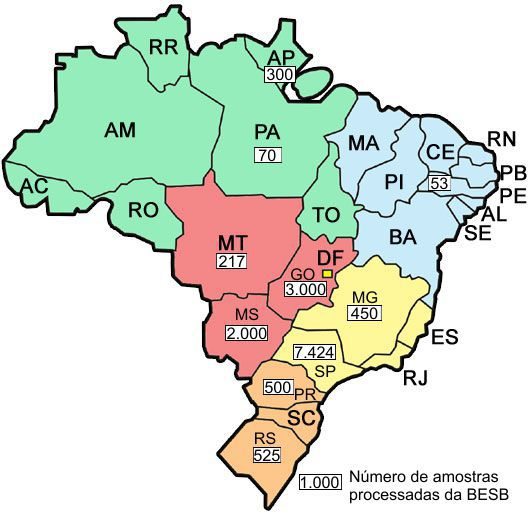
\includegraphics[width=0.8\textwidth]{figuras/brasil.jpg}
   \caption{Mapa do Brasil com a distribuição do número de amostras processadas por estado da Biblioteca Espectral de Solos do Brasil - BESB.}
   \label{fig:brasil}
\end{figure}

A biblioteca da ESALq armazena dezenas de artigos, dissertações e teses disponíveis em \url{http://esalqgeocis.wix.com/geocis}. Além disso, todos os dados gerais sobre o banco de dados e artigos específicos em espectrorradiometria encontram-se em \url{http://bibliotecaespectral.wix.com/esalq}.

\begin{footnotesize}
\begin{thebibliography}{99}

\bibitem[FAO(2013) FAO]{FAO:2013}
FAO (2013)
\newblock {\em State of the Art Report on Global and Regional Soil Information: Where are we? Where to go?}
\newblock Rome: FAO.

\bibitem[Brasil(2013) Brasil]{Brasil:2013}
Brasil (2013)
\newblock {\em Projeções do Agronegócio: Brasil 2012/2013 a 2022/2023.}
\newblock Disponível em \url{http://www.agricultura.gov.br/arq\_editor/projecoes\%20-\%20versao\%20atualizada.pdf}.

\bibitem[Mahmood(1987) Mahmood]{Mahmood:1987}
K. Mahmood (1987)
\newblock {\em Reservoir sedimentation - impact, extent and mitigation.}
\newblock Washington: World Bank.

\bibitem[Lal(2003) Lal]{Lal:2003}
R. Lal (2003)
\newblock Soil erosion and the global carbon budget.
\newblock {\em Environment International}, 29:437-450.

\bibitem[Singh \& Ghoshal(2010) Singh, Ghoshal]{SinghEtAl:2010}
P. Singh, N. Ghoshal (2010)
\newblock Variation in total biological productivity and soil microbial biomass in rainfed agroecosystems. Impact of application of herbicide and soil amendments.
\newblock {\em Agric. Ecosyst. Environ}, 137:241-250.

\bibitem[Coelho et~al.(2013) Coelho, Barbalho, Escremin]{CoelhoEtAl:2013}
A. Coelho, E.S. Barbalho, J.V. Escremin (2013)
\newblock Desenvolvimento de um experimento sobre o efeito estufa: uma proposta para o ensino.
\newblock {\em Rev. Virtual Quim}, 6:142-151.

\bibitem[Lal(1999) Lal]{Lal:1999}
R. Lal (1999)
\newblock {\em Métodos para a avaliação do uso sustentável dos recursos solo e água nos trópicos.}
\newblock Jaguariúna: Embrapa Meio Ambiente.

\bibitem[Mendonça-Santos \& Santos(2007) Mendonça-Santos, Santos]{Mendonca-SantosEtAl:2007}
M.L. Mendonça-Santos, H.G. Santos (2007)
\newblock The state of the art of brazilian soil mapping and prospects for digital soil mapping.
\newblock {\em Developments in soil science}, 31:39-54.

\bibitem[Soriano-Disla et~al.(2014) Soriano-Disla, Janik, Viscarra Rossel, Mac Donald, McLaughlin]{Soriano-DislaEtAl:2014}
J.M. Soriano-Disla, L.J. Janik, R.A. Viscarra Rossel, L.M. Mac Donald, M.J. McLaughlin (2014)
\newblock The performance of visible, near-, and mid-infrared reflectance spectroscopy for prediction of soil physical, chemical, and biological properties.
\newblock {\em Applied Spectroscopy Reviews}, 49:139-186.

\bibitem[Vasques et~al.(2014) Vasques, Demattê, Ramirez Lopes, Terra]{VasquesEtAl:2014}
G.M. Vasques, J.A.M. Demattê, L. Ramirez Lopes, F.S. Terra (2014)
\newblock Soil classification using visible/near-infrared diffuse reflectance spectra from multiple depths.
\newblock {\em Geoderma}, \textit{in press}.

\bibitem[Stoner \& Baumgardner(1981) Stoner, Baumgardner]{StonerEtAl:1981}
E.R. Stoner, M.F. Baumgardner (1981)
\newblock Characteristic variations in reflectance of surface soils.
\newblock {\em Soil Sci. Soc. Amer. J.}, 45:1161-1165.

\bibitem[Shepherd \& Walsh(2002) Shepherd, Walsh]{ShepherdEtAl:2002}
K.D. Shepherd, M.G. Walsh (2002)
Development of reflectance spectral libraries for characterization of soil properties. Soil Science Society of America Journal, v.66, p.988-998.

\bibitem[Brown et~al.(2006) Brown, Shepherd, Walsh, Mays, Reinsch]{BrownEtAl:2006}
D.J. Brown, K.D. Shepherd, M.G. Walsh, M.D. Mays, T.G. Reinsch (2006)
\newblock Global soil characterization with VNIR diffuse reflectance spectroscopy.
\newblock {\em Geoderma}, 132:273-290.

\bibitem[Epiphânio et~al.(1992) Epiphânio, Formaggio, Valeriano, Oliveira]{EpiphanioEtAl:1992}
J.C.N. Epiphânio, A.R. Formaggio, M.M. Valeriano, J.B. Oliveira (1992)
\newblock {\em Comportamento espectral de solos do Estado de São Paulo.}
\newblock José dos Campos: INPE.

\bibitem[Formaggio et~al.(1996) Formaggio, Epiphanio, Valeriano, Oliveira]{FormaggioEtAl:1996}
A.R. Formaggio, J.C.N. Epiphanio, M.M. Valeriano, J.B. Oliveira (1996)
\newblock Comportamento espectral (4502.450 nm) de solos tropicais de São Paulo.
\newblock {\em Revista Brasileira de Ciência do Solo}, 20:467-474.

\bibitem[Bellinaso et~al.(2010) Bellinaso, Dematte, Romeiro]{BellinasoEtAl:2010}
H. Bellinaso, J.A.M. Dematte, S.A. Romeiro (2010)
\newblock Soil spectral library and its use in soil classification.
\newblock {\em R. Bras. Ci. Solo}, 34:861-870.

\bibitem[Demattê et~al.(2004) Demattê, Campos, Alves, Fiorio, Nanni]{DematteEtAl:2004}
J.A.M. Demattê, R.C. Campos, M.C. Alves, P.R. Fiorio, M.R. Nanni (2004)
\newblock Visible-NIR reflectance: a new approach on soil evaluation.
\newblock {\em Geoderma}, 121:95-112.

\bibitem[Demattê et~al.(2001) Demattê, Demattê, Camargo, Fiorio, Nanni]{DematteEtAl:2001}
J.A.M. Demattê, J.L.I. Demattê, W.P. Camargo, P.R. Fiorio, M.R. Nanni (2001)
\newblock Remote sensing in the recognition and mapping of tropical soils developed on topographic sequences.
\newblock {\em Mapping Sciences and Remote Sensing}, 38:79-102.

\bibitem[Odlare et~al.(2005) Odlare, Svensson, Pell]{OdlareEtAl:2005}
M. Odlare, K. Svensson, M. Pell (2005)
\newblock Near intrared reflectance spestrocopy for assessement of spatial soil variation in an agricultural field.
\newblock {\em Geoderam}, 126:193-202.

\bibitem[Thomasson et~al.(2001) Thomasson, Sui, Cox, Al-Rajehy]{ThomassonEtAl:2001}
J.A. Thomasson, R. Sui, M.S. Cox, A. Al-Rajehy (2001)
\newblock Soil reflectance sensing for determining soil properties in precision agriculture.
\newblock {\em Trans. Am. Soc. Agron. Eng.}, 44:1445-1453.

\bibitem[Viscarra Rossel(2009) Viscarra Rossel]{ViscarraRossel:2009}
R.A. Viscarra Rossel (2009)
\newblock The Soil Spectroscopy Group and the development of a global soil spectral library.
\newblock {\em EGU General Assembly Conference Abstracts}, 11:14021.

\end{thebibliography}
\end{footnotesize}

\address{José Alexandre M. Demattê\\
  Departamento de Ciência do Solo, ESALQ/USP\\
  \email{jamdemat@usp.br}}
  
\address{Marilusa P. C. Lacerda\\
  Faculdade de Agronomia e Medicina Veterinária, FAV/UnB\\
  \email{marilusa@unb.br}}
%%% Local Variables: 
%%% mode: latex
%%% TeX-master: 4th-edition.tex
%%% End: 